\chapter{VM design}
\section{Ahead-of-Time translation}
\label{sec-aot-translation}
Our implementation is based on Darjeeling \cite{Brouwers:2009cj}, a Java VM for sensor nodes, running on an Atmel ATmega CPU. Like other sensor node VMs, it is originally an interpreter. We add an AOT compiler to Darjeeling: instead of interpreting the bytecode, the VM translates it to native code at load time, before the application is started. While JIT compilation is possible on some devices \cite{Ellul:2012thesis}, it depends on the ability to execute code from RAM, which many embedded CPUs, including the ATmega, cannot do.

\begin{figure}[]
  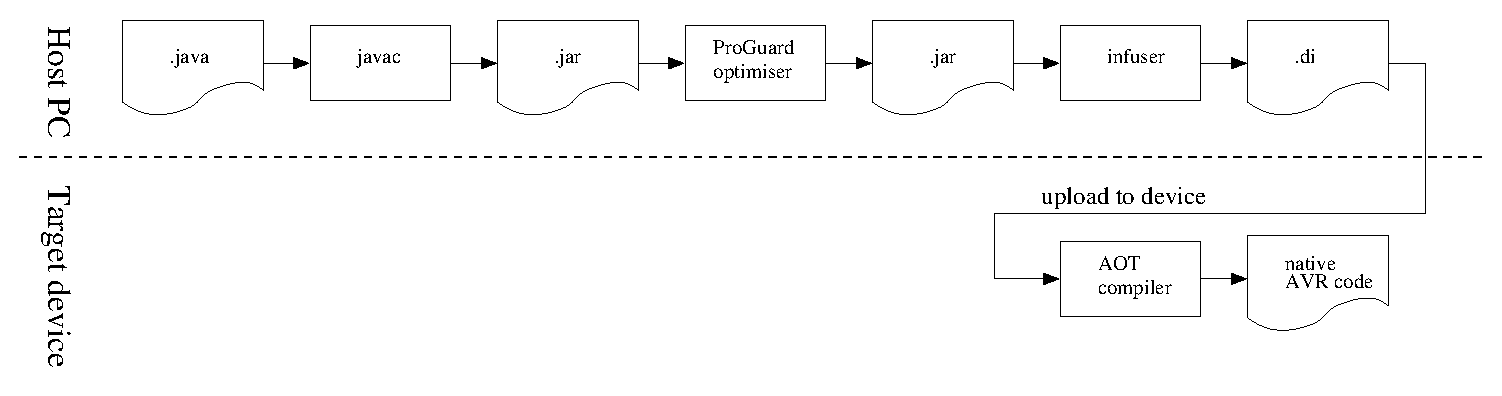
\includegraphics[width=\linewidth]{compilation-process.eps}
  \caption{Java to native AVR compilation}
  \label{fig-translation-process}
\end{figure}

% TODO: clarify two terms: compile-time (javac/proguard/infuser) and translation-time (the VM), and scan the whole text to make sure they're used consistently.

The process from Java source to a native application on the node is shown in Figure \ref{fig-translation-process}. Like all sensor node JVMs, Darjeeling uses a modified JVM bytecode. Java source code is first compiled to normal Java classes, which are optimised by ProGuard \cite{proguard}. The optimised Java classes are then transformed into Darjeeling's own format, called an 'infusion'. For details of this transformation we refer to the Darjeeling paper \cite{Brouwers:2009cj}. Here it is sufficient to know that the bytecode is modified to make it more suitable for execution on a tiny device, for example by adding 16-bit versions of most operations, but the result remains very similar to standard JVM bytecode. It is also important to note that no knowledge of the target platform is used in this transformation, so the result is still platform independent. This infusion is then sent to the node, where it is translated to native AVR code at load time.

We made several modifications to Darjeeling's infuser and bytecode format to support our AOT compiler and improve performance. These changes will be introduced in more detail in the following sections, but for completeness we also list them here:

\begin{itemize}
	\item the \mycode{BRTARGET} opcode, used to mark targets of branch instructions and modified all branch instructions to target a \mycode{BRTARGET} id instead of a bytecode offset
	\item the \mycode{MARKLOOP} opcode to mark inner loops and the variables it uses
	\item added \mycode{\_FIXED} versions of the \mycode{GETFIELD\_A} and \mycode{PUTFIELD\_A} opcodes, used to access an object's reference fields when the offset is known at compile time
	\item the \mycode{SIMUL} opcode for 16x16-bit to 32-bit multiplication
	\item modified array access opcodes to use 16-bit indexes
	\item added \mycode{\_CONST} versions of the bit shift opcodes to support constant shifts
	\item the \mycode{INVOKELIGHT} opcode for an optimised 'lightweight' way of calling methods
\end{itemize}

\subsection{Goals and limitations}
Working on resource-constrained devices means we have to make some compromises. Our main goal is to build a VM that will produce code that both performs well, and adds as little code size overhead as possible. In addition, we want our VM to fit as many scenarios as possible. We would like to be able to support scenarios were multiple applications may be running on a single device, so when new code is being loaded, the impact on other applications should be as small as possible.

Therefore, the translation process should be very light weight. Specifically, it	 should use as little memory as possible, since memory is a very scarce resource. This means we cannot do any analysis on the bytecode that would require us to hold complex data structures in memory. When receiving a large programme, we should not have to keep multiple messages in memory, but will free each message, which can be as small as a single JVM instruction, immediately after processing.

Since messages do need to be processed in the correct order, the actual transmission protocol may still decide to keep more messages in memory to reduce the need for retransmissions in the case of out of order delivery. But our translation process does not require it to do so, and a protocol that values memory usage over retransmissions cost could simply discard out of order messages and request retransmissions when necessary.

Bytecode instructions are processed in a single pass, one instruction at a time. Only some small, fixed-size data structures are kept in memory during the process. A second pass over the generated code then fills in addresses left blank by branch instructions, since the target addresses of forward branches are not known until the target instruction is generated.

The two metrics we compromise on are load time and code size. Compiling to native code takes longer than simply storing bytecode and starting the interpreter, but we feel this load time delay will be acceptable in many cases, and will be quickly compensated for by improved run-time performance. Native code is also larger than JVM bytecode. This is the price we pay for increased performance, but the optimisations we propose do significantly reduce this code size overhead compared to previous work, thus reducing an important drawback of AOT compilation.

Since our compiler is based on Darjeeling, we share its limitations, most notably a lack of floating point support and reflection. In addition, we do not support threads or exceptions because after compilation to native code, we lose the interpreter loop as a convenient place to switch between threads or unwind the stack to jump to an exception handler. Threads and exceptions have been implemented before on a sensor node AOT compiler \cite{Ellul:2012thesis}, proving it is possible to add support for both, but we feel the added complexity in an environment where code space is at a premium makes other, more lightweight models for concurrency and error handling more appropriate.

\subsection{Translating bytecode to native code}
\label{sec-basic-translation}
The basic approach to translate bytecode to native code on a sensor node was first described by Ellul and Martinez \cite{Ellul:2010iw}. When we receive a bytecode instruction, we simply replace it with an equivalent sequence of native instructions, using the native stack to mimic the JVM stack. An example is shown in Table 1.

The first column shows a fragment of JVM code which does a shift right of variable \mycode{A}, and repeats this while \mycode{A} is greater than \mycode{B}. While not a very practical function, it is the smallest example that will allow us to illustrate our code generation optimisations. The second column shows the code the AOT compiler will execute for each JVM instruction. Together, the first and second column match the case labels and body of a big switch statement in our compiler. The third column shows the resulting AVR native code, which is currently almost a 1-on-1 mapping, with the exception of the branch and some small optimisations by a simple peephole optimiser, both described below.

The example has been slightly simplified for readability. Since the AVR is an 8-bit CPU, in the real code many instructions are duplicated for loading the high and low bytes of a short. The cycle count is based on the actual number of generated instructions, and for a single iteration.

\begin{table}[]
\centering
\caption{Translation of \mycode{ do\{A{>}{>}{>}=1;\} while(A>B);}}
\label{tbl-basic-translation}
\small
\begin{tabular}{llll}
\toprule
JVM & AOT compiler & AVR & cycles \\
\hline
0: BRTARGET(0)   & \sccomment{record current addr} &                &   \\
1: SLOAD\_0      & emit\_LDD(R1,Y+0)        & LDD R1,Y+0     & 4 \\
                 & emit\_PUSH(R1)           & PUSH R1        & 4 \\
2: SCONST\_1     & emit\_LDI(R1,1)          & LDI R1,1       & 2 \\
                 & emit\_PUSH(R1)           & MOV R2,R1      & 1 \\
3: SUSHR         & emit\_POP(R2)            &                &   \\
                 & emit\_POP(R1)            & POP R1         & 4 \\
                 & emit\_RJMP(+2)           & RJMP +2        & 2 \\
                 & emit\_LSR(R1)            & LSR R1         & 2 \\
                 & emit\_DEC(R2)            & DEC R2         & 2 \\
                 & emit\_BRPL(-2)           & BRPL -2        & 3 \\
                 & emit\_PUSH(R1)           &                &   \\
4: SSTORE\_0     & emit\_POP(R1)            &                &   \\
                 & emit\_STD(Y+0,R1)        & STD Y+0,R1     & 4 \\
5: SLOAD\_0      & emit\_LDD(R1,Y+0)        & LDD R1,Y+0     & 4 \\
                 & emit\_PUSH(R1)           & PUSH R1        & 4 \\
6: SLOAD\_1      & emit\_LDD(R1,Y+2)        & LDD R1,Y+2     & 4 \\
                 & emit\_PUSH(R1)           &                &   \\
7: IF\_SCMPGT 0: & emit\_POP(R1)            &                &   \\
                 & emit\_POP(R2)            & POP R2         & 4 \\
                 & emit\_CP(R1,R2)          & CP R1,R2       & 2 \\
                 & emit\_branchtag(GT,0)    & BRGT 0:        & 2 (taken), \\
                 &                          &                & or 1 (not taken) \\
\bottomrule
\end{tabular}
\end{table}

\subsubsection{Peephole optimisation}
From Table \ref{tbl-basic-translation} it is clear that this approach results in many unnecessary push and pop instructions. Since the JVM is a stack-based VM, each instruction must obtain its operands from the stack and push any result back onto it. As a result, almost half the instructions are push or pop instructions.

To reduce this overhead, Ellul proposes a simple peephole optimiser \cite{Ellul:2012thesis}. The compilation process results in many push instructions that are immediately followed by a pop. If they target the same register, they have no effect and are removed. If the source and destination registers differ, the two instructions are replaced by a move. The result is shown in the third column of Table \ref{tbl-basic-translation}. Two push/pop pairs have been removed, and one has been replaced by a move.

\subsubsection{Branches}
Forward branches pose a problem for our direct translation approach since the target address is not yet known. A second problem is that on the ATmega, a branch may take 1 to 3 words, depending on the distance to the target, so it is also not known how much space should be reserved for a branch.

To solve this the infuser modifies the bytecode by inserting a new instruction, \mycode{BRTARGET}, in front of any instruction that is the target of a branch. The branch instructions themselves are modified to target a branch target id instead of a bytecode offset. When we encounter a \mycode{BRTARGET} during compilation, we do not emit any code, but record the address where the next instruction will be emitted in a separate part of flash. When we encounter a branch instruction, we emit a temporary 3-word 'branch tag' instead, containing the branch target id and the branch condition. After code generation is finished and all target addresses are known, we scan the code again to replace each branch tag with the real branch instruction.

There is still the matter of the different sizes a branch may take. We could simply add \mycode{NOP} instructions to smaller branches to keep the size of each branch at 3 words, but this causes a performance penalty on small, non-taken branches. Instead, we do another scan of the code, before replacing the branch tags, and update the branch target addresses to compensate for cases where a smaller branch will be used. This second scan adds about 500 bytes to the VM, but improves performance, especially on benchmarks where branches are common.

This is an example of something we often see: an optimisation may take a few hundred bytes to implement, but its usefulness may depend on the characteristics of the code being run. In this work we usually decided to implement these optimisations, since they often also result in smaller generated code.

\subsection{Darjeeling split-stack architecture}
\label{sec-darjeeling-split-architecure}
\begin{figure}[]
  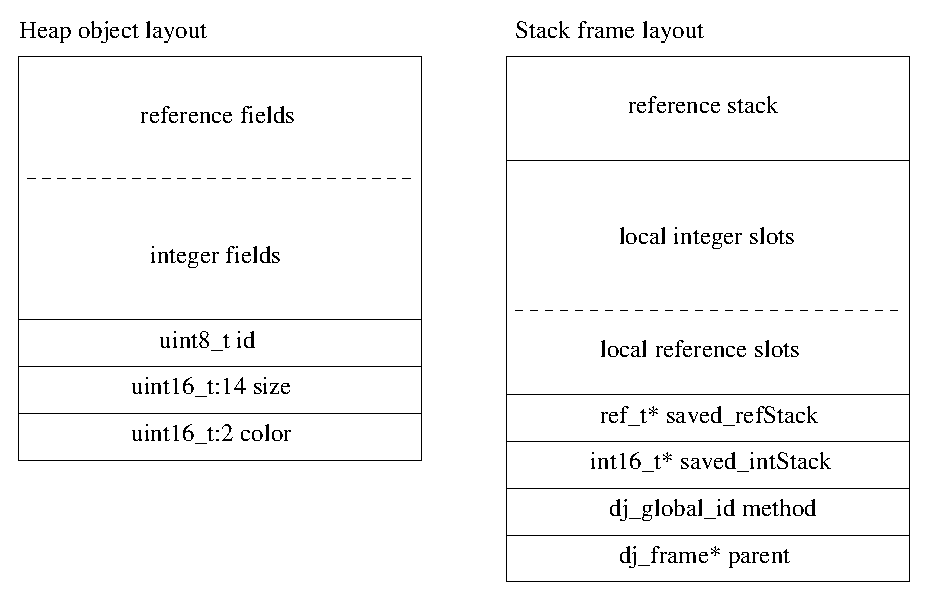
\includegraphics[width=0.5\linewidth]{object-and-stack-frame-layout.eps}
  \caption{Object and stack frame layout}
  \label{fig-object-and-stack-frame-layout}
\end{figure}

In Darjeeling, reference and integer values are separated throughout the VM. When the garbage collection runs, it needs to determine which stack values, local variables, static variables and object fields are references. To handle this efficiently, Darjeeling splits references and integers in all these cases, as shown in Figure \ref{fig-object-and-stack-frame-layout}.

In our AOT compiler we use the native stack for the JVM integer operand stack, while space for the reference stack is reserved in the stack frame. This uses less memory than having the integer stack in the stack frame, since we need to reserve space for the maximum stack depth in the frame, which is often much lower for the reference stack than for the integer stack. We use the AVR's X register as a stack pointer for the reference stack.

\subsection{Target platforms}
The AVR family of CPUs is widely used in low power embedded systems. We implemented our VM for the ATmega128 CPU. However, our approach does not depend on any AVR specific properties and we expect similar results for many other CPUs in this class. The main requirements are the ability to reprogramme its own programme memory, and the availability of a sufficient number of registers.

The ATmega128 has 32 8-bit registers. We ran several experiments where we restrict the number of registers our VM may use. As is often the case with caches, we found the first few available registers to have the largest impact, while the added improvement gets less for each added register. Based on this we expect the Cortex M0, with 12 32-bit general purpose registers, or the MSP430, with 12 16-bit registers, and used by Ellul and Martinez \cite{Ellul:2010iw}, to both be good matches as well.

%TODO: references for M0 and MSP430?







